\documentclass{standalone}

\usepackage[latin1]{inputenc}
\usepackage{tikz}

\usetikzlibrary{calc}

% GNUPLOT required
\begin{document}
\pagestyle{empty}

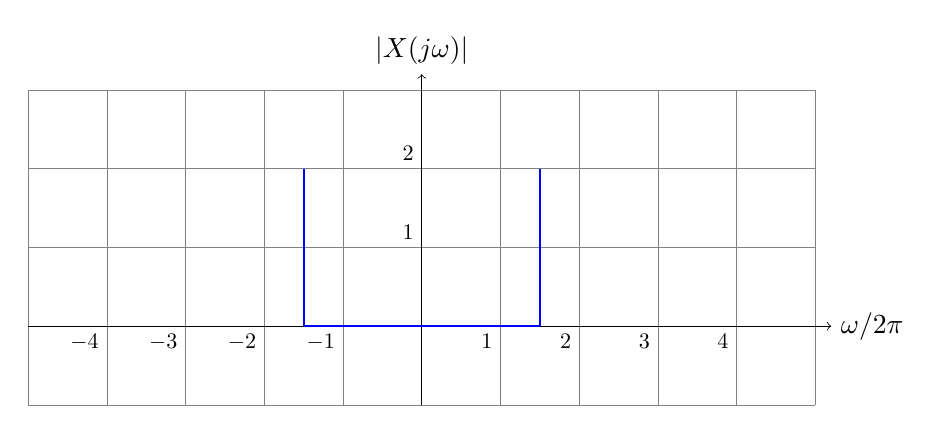
\begin{tikzpicture}[line width=0.25mm]
    \draw[very thin,color=gray] (-5,-1) grid (5,3);
    \draw[->, line width=0.1mm] (-5,0) -- (5.2,0) node[right] {$\omega/2\pi$};
    \draw[->, line width=0.1mm] (0,-1) -- (0,3.2) node[above] {$|X(j\omega)|$};

	% x(t)
    \draw[color=blue, domain=-5:-3.5] plot[id=x] function{0};
    \draw[color=blue, domain=-3.5:-1.5] plot[id=x] function{x+3.5};
	\draw[color=blue] (-1.5,2) -- (-1.5,0);
    \draw[color=blue] (-1.5,0) -- (1.5,0);
	\draw[color=blue] (1.5,2) -- (1.5,0);
    \draw[color=blue, domain=3.5:1.5] plot[id=x] function{-x+3.5};
    \draw[color=blue, domain=5:3.5] plot[id=x] function{0};% Para indicar la fucnción, se puede quitar los comentario y el último ;
        %node[above right] {$x(t)$};


	\foreach \x in {-4,...,-1,1,2,...,4} {%
    \draw ($(\x,0) + (0,0)$) -- ($(\x,0) + (0,0)$)
        node [below left,scale=0.8] {$\x$};
	}
	\foreach \y in {1,2} {%
    \draw ($(0,\y) + (0,0)$) -- ($(0,\y) + (0,0)$)
        node [above left,scale=0.8] {$\y$};
	}

\end{tikzpicture}


\end{document}
